%!TEX root = ../report.tex
%*******************************************************************************
%                              Design & Hardware                               %
%*******************************************************************************


\chapter{Design \& Hardware}

%******************************** Section 4.1 *********************************%
\section{Introduction}
    Once the system requirements are identified, the next step would be to prepare the conceptual representation
    of the project. This part focuses just on the worker, specifying its requirements and going all the way
    from the software and the communication with the scheduler to the hardware specifications.

%******************************** Section 4.2 *********************************%
\section{Design and technical specifications}

    The following diagram presents the interaction between the different components of the worker.
    The connection between the components is guaranteed by the TCP protocol.
    The ports 4321, 4322, 4323 and 4324 should be open in both machines, the worker and the scheduler.
    At the start-up, the worker downloads the CA certificate. This part is mandatory for the program
    to continue working.

    \clearpage

    \begin{figure}[!h]\centering
        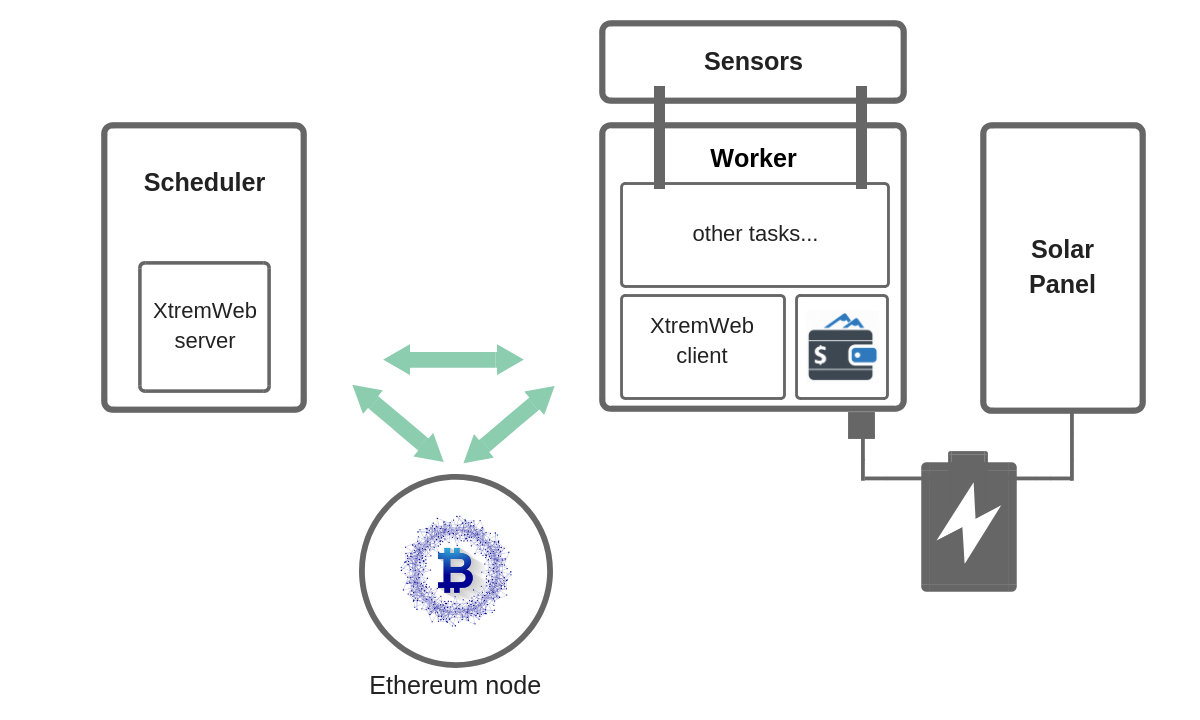
\includegraphics[width=.9\columnwidth]{5-Design/figs/worker-diagram.png}
        \caption{Global overview of the worker design}
    \end{figure}

    We explain in the following subsections the role and requirements of each
    component.

    \subsection{Worker}

        \begin{figure}[!h]\centering
            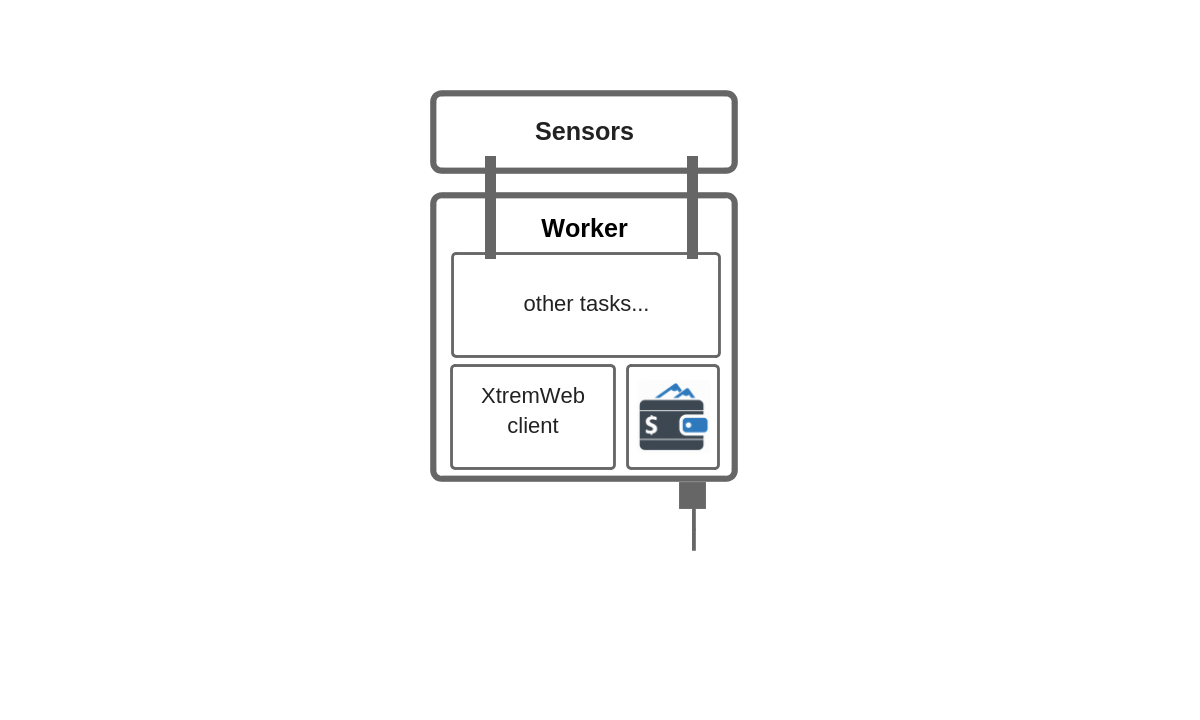
\includegraphics[width=.9\columnwidth]{5-Design/figs/worker.png}
            \caption{The worker internal sortware components}
        \end{figure}

        % \begin{figure}[!h]\centering
        %     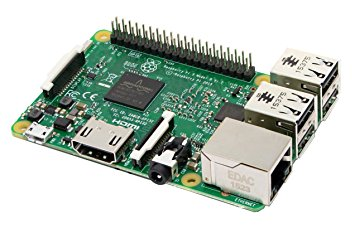
\includegraphics[width=.4\columnwidth]{5-Design/figs/raspberry.jpg}
        %     \caption{The worker internal sortware components}
        % \end{figure}

        The worker runs a docker image of XtremWeb worker. This image has to be optimized for devices with
        limited resources like the Raspberry Pi board.
        XtremWeb does not support ARM architecture natively so this support should be introduced
        to the new version of the middleware. Luckily docker is available for this architecture which simplifies
        the task.

    \subsection{Blockchain}
    
        \begin{figure}[!h]\centering
            \includegraphics[width=.3\columnwidth]{5-Design/figs/blockchain-logo.png}
            \caption{The solar panel}
        \end{figure}

        The blockchain part is represented by the Geth node where we deploy the iExec smart contracts.
        The worker should take care of the necessary blokchain configuration for the proper functioning
        of the system, so it should provide a wallet with sufficient funds (in RLC). The scheduler locks
        an amount of RLC when an execution is starting, so the worker should have the minimum amount
        required by the operation. If these requirements are not satisfied the program will crash.

    \subsection{Use case diagram}
        Use case diagram describes the functionality provided by a system in terms of actors, their
        goals represented as use cases, and any dependencies among those use cases.
        It is therefore to have an external view of the functioning of the system, which on the one hand
        defines the behavior of the system in its environment and on the other hand to identify the needs
        and objectives expected of the actors. At this stage we're going to focus on the worker as our
        system. \newline
        At first we start by introducing the interacting actors, then we present a description about
        functionalities provided. \newline \newline
        \textit{Actors: }
        An actor represents a role played by an external entity that directly interacts with the system
        being studied. Our actors are:
        \begin{itemize}
            \item \textbf{The scheduler: }
            it sends jobs to the worker, waits for the execution to finish, verifies the results and does
            the payment transactions.
            \item \textbf{The external service: }
            This actor does not have effect on the system (worker). It receives the data sent by the worker.
            \item \textbf{The solar panel: }
            It provides the necessary energy for the worker.
        \end{itemize}
        \textit{Use cases: }
        A use case represents a set of action sequences that are performed by the system and that produce
        an observable result of interest for a particular actor.

        \begin{itemize}
            \item \textbf{Scheduler}
                \begin{itemize}
                    \item Delegate jobs: the scheduler sends the description of received tasks to the worker
                    to execute it.
                    \item Get the result of execution: after the execution the worker sends the result back
                    to the scheduler.
                    \item Pay execution: the scheduler sends the reward to the worker.
                \end{itemize}
            
            \item \textbf{External service}
                \begin{itemize}
                    \item Subscribe to data stream: The service subscribes to receive the data.
                    \item Receive processed data stream: The service receives the collected data sent by the
                    worker.
                \end{itemize}
            
            \item \textbf{Solar panel}
                \begin{itemize}
                    \item Implement the energy produced: the panel supplies the worker with the necessary energy.
                \end{itemize}
        \end{itemize}


        \begin{figure}[!h]\centering
            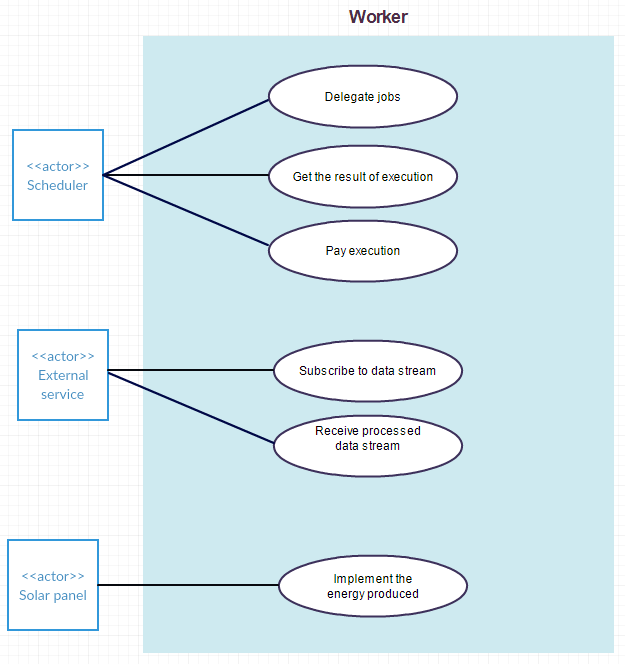
\includegraphics[width=\columnwidth]{5-Design/figs/use-case-diagram.png}
            \caption{Worker use case diagram}
        \end{figure}

        \clearpage

%******************************** Section 4.3 *********************************%
\section{Hardware}

    \subsection{Solar Panel}

        \begin{figure}[!h]\centering
            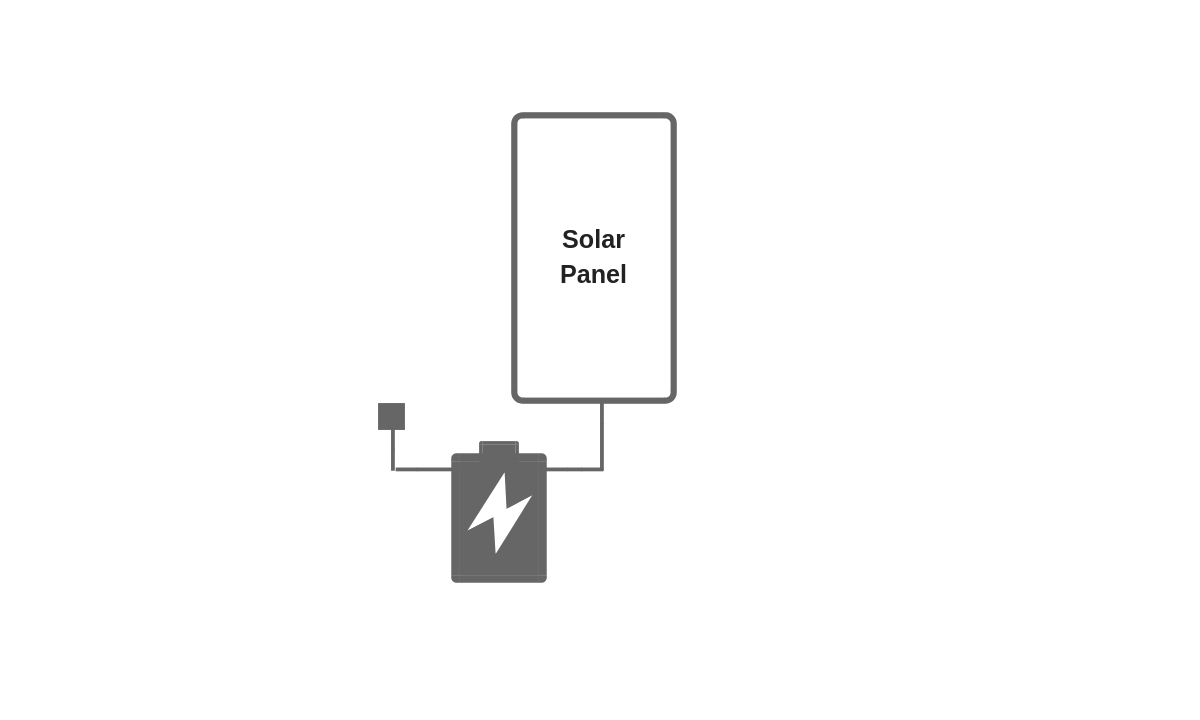
\includegraphics[width=.6\columnwidth]{5-Design/figs/solar-panel.png}
            \caption{The solar panel}
        \end{figure}

        A Photovoltaic solar panels is used to power the worker. It absorbs sunlight as a source of energy to
        generate electricity and charge the battery. In this case we use a panel with high conversion
        efficiency: 60 watt SUNPOWER mono-crystalline with conversion efficiency up to 25\% which is much
        higher than common solar panel charger (15\%).

        Reference of the chosen panel: SUAOKI 60W Portable Sunpower Mono-crystalline Solar Panel with DC 18V and USB
        5V Output Charger.\newline
        Output: up to 60W - USB: 18v/3.4A, DC: 5v/2.5A.

        \begin{figure}[!h]\centering
            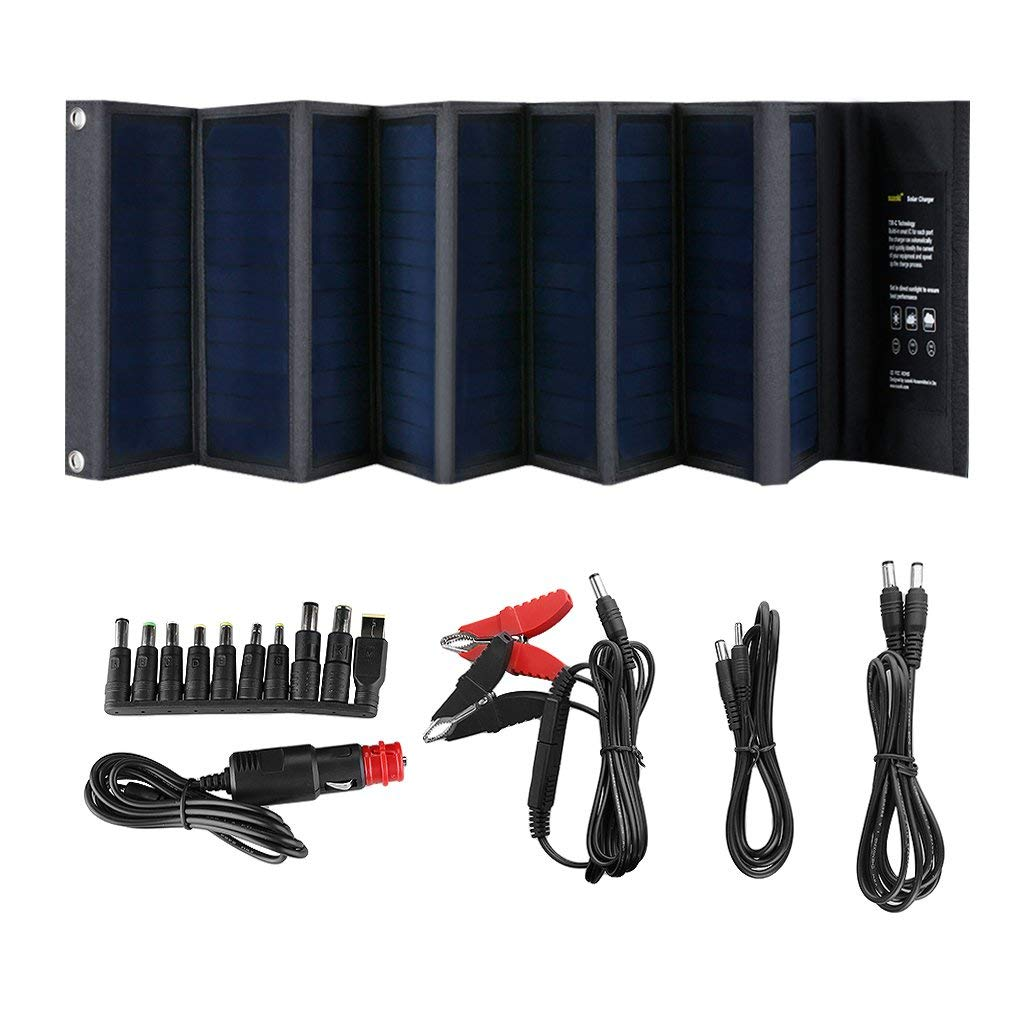
\includegraphics[width=.4\columnwidth]{5-Design/figs/panel.jpg}
            \caption{SUNPOWER solar panel}
        \end{figure}

        This panel should be able to charge the battery in merely 8 hours during a sunny day. The Raspberry
        Pi board consumes 1A for a maximum utilization of the CPU and some plugged sensors. For a battery
        capacity of 50000mA, the worker can stay up for 24 hours for a full battery without any source of
        solar light.

    \subsection{Battery}

        \begin{figure}[!h]\centering
            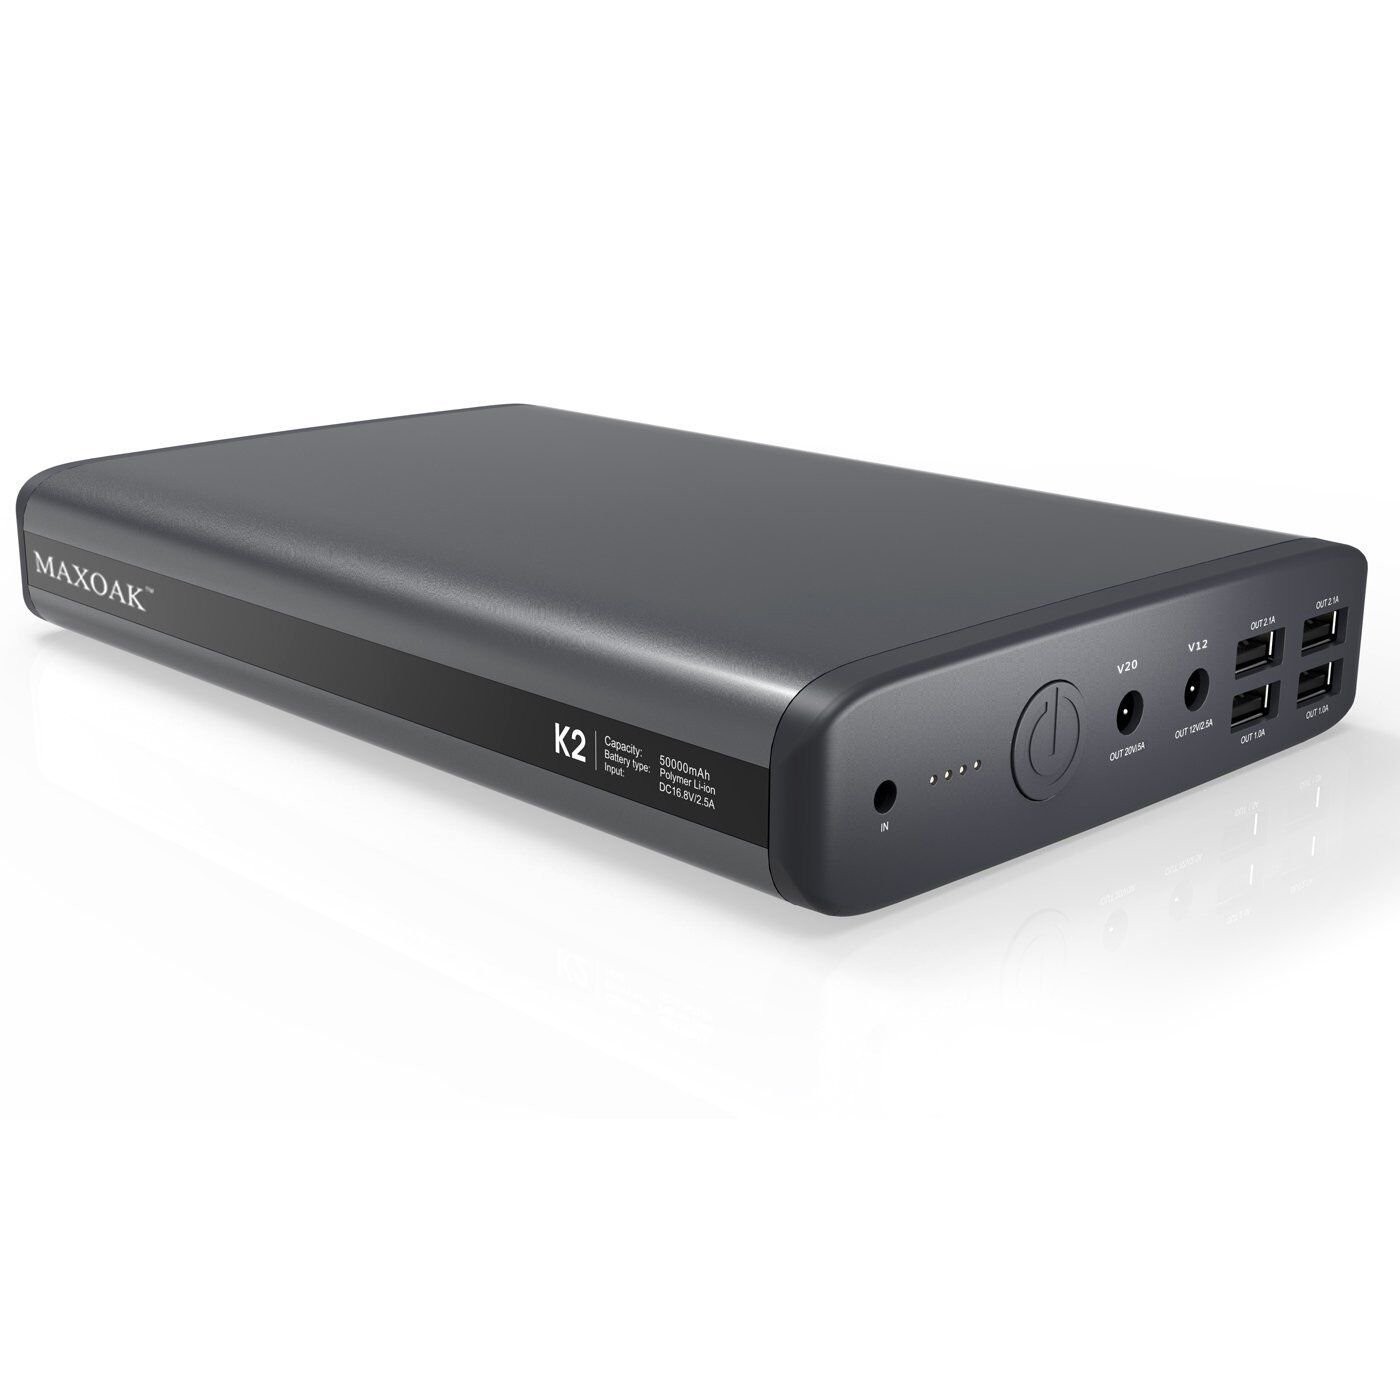
\includegraphics[width=.3\columnwidth]{5-Design/figs/battery.jpg}
            \caption{50000 mA Battery}
        \end{figure}

        We suppose that the battery should be able to store electricity for, at least, two days. With a
        consumption of maximum 24A/day, the battery should store 50A. It should also contain a 5V output
        to power the worker with the right intensity.

        Reference of the chosen battery: MAXOAK 50000mAh 5/12/20v Portable Charger External Battery Power Bank.

    \subsection{Sensors}
        The worker uses different sensors to interact with the outside world. We can imagine multiple systems
        with a lot of use cases. We will take as example two use cases:

        \underline{Surveillance camera:} the worker has an 8 megapixel native resolution sensor-capable of 3280 x 2464
        pixel static images camera to achieve the mission of a surveillance system that streams video and detects motions.

        \begin{figure}[!h]\centering
            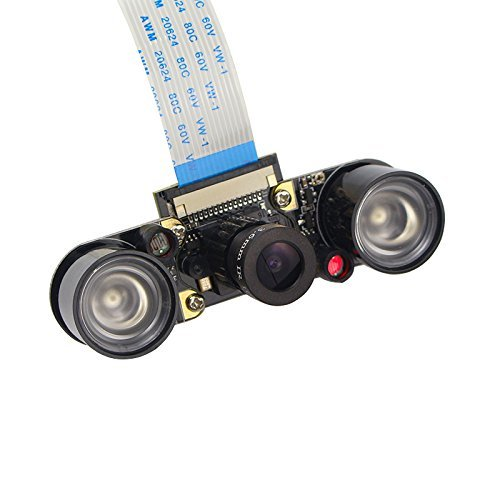
\includegraphics[width=.2\columnwidth]{5-Design/figs/camera.jpg}
            \caption{Raspberry Pi camera}
        \end{figure}


        \underline{Weather station:} in this case the worker uses a humidity, pressure, temprature and
        orientation senors to build a weather station. It collects weather data and applies some
        processing on it before sending it to a weather forcast service. The data processing can be done
        with an iExec dapp locally on the worker and this model has many advantges such as pushing the
        processing to the edge of the network to reduce latency caused by data transfer and enhance data
        privacy because it is not leaving the device.

        \begin{figure}[!h]\centering
            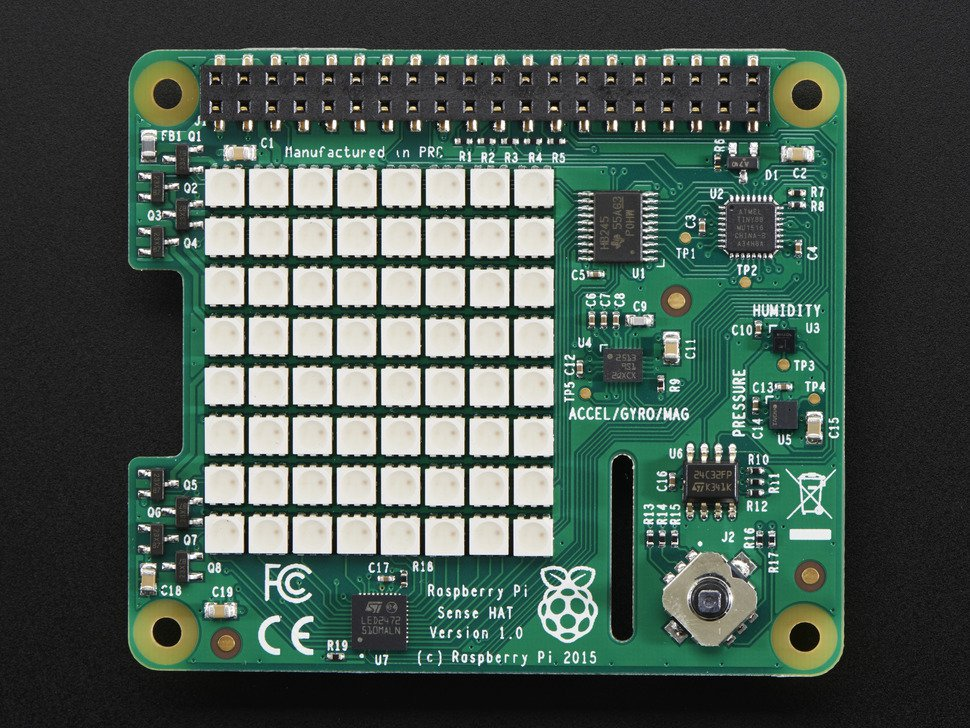
\includegraphics[width=.3\columnwidth]{5-Design/figs/sense-hat.jpg}
            \caption{Raspberry Pi Sense HAT}
        \end{figure}

%******************************** Section 4.4 *********************************%
\section{Conclusion}
    In this chapter, we worked on the first place on designing the worker taking in consideration the resources
    limitation of the worker board. In the second section, we worked on choosing the hardware that suits
    the requirements, therefore we pass to the implementation part to shape our design.